\chapter{Bitcoin security concerns}
\label{sec:securityintro}

Bitcoin's decentralized, uncontrolled environment is open to a wide range of attacks, many of which are common threats for other cryptocurrencies as well. For this reason, the attacks described here can be carried out on other systems as well. These attacks have the same rationale, but different implementations.\\

Decentralized permissionless blockchains with PoW-based consensus algorithms are by definition vulnerable to \textit{51\%} or \textit{majority} attacks~\cite{nakamoto}. In these a user controls more than half of the computing power (often called \textit{hash rate}) available on the entire network~\cite{51atk}.

The attacker can thus subvert the consensus algorithm and validate harmful data, maliciously fork the blockchain or arbitrarily prevent blocks and transactions from verification.\\

Most of the malicious users that aim for a revenue from their attacks opt for \textit{double-spending} attacks. By definition, in double-spending attacks the same set of outputs is spent twice, hence the attacker gains Bitcoins or obtains resources from merchants for free.

Although proof-of-work consensus makes double-spending infeasible, since the transactions would not be validated, the attack can be still executed through other approaches. As a case in point, double-spending can be executed  if the attacker can successfully partition the network (see Section~\ref{sec:sybil}, or were other conditions to be met~\cite{doublespendfastpay}).\\

The way the correct state of the blockchain is elected, selecting the longest branch as the only valid, is exploitable for attacks that engineer block races.

In block races two or more peers spend computing power mining different forks of the same height. By definition of Bitcoin's consensus, there will be a point at which only one branch will be selected as valid and all the others will be discarded.

Block races can enable double-spending, as shown in Section~\ref{sec:sybil} and~\ref{sec:eclipse}, or mining attacks such as \textit{selfish mining}, where the malicious user holds private his mined blocks, thus forking the chain.

For the time the private chain of the attacker is longer that the public one, it can be released on the network, thus claiming the rewards for himself and wasting other miners' computing power~\cite{selfishmining}.\\

Since this chapter serves only introductory purposes, these are just a few attacks that can be driven onto Bitcoin. In the following sections there is more on network attacks, which are the focus of this thesis. The interested reader can find complete security overviews in the works of Conti et al., Saad et al. and Wang et al.~\cite{contiatksurvey},~\cite{saad2019attacksurface},~\cite{secpermissionlessblock}.

\section{Network security}\label{sec:netsec}
Attacks that exploit vulnerabilities in the design and implementation of the Bitcoin protocol and its peer-to-peer network fall under the category of network attacks.

Bitcoin is exposed to all the common threats that affect other peer-to-peer systems; these have been widely studied in the literature as in Touceda et al, 2012~\cite{toucedafakeboot}. The aim of this section is to understand how these attacks apply to Bitcoin and what are its defences\\

In network attacks. often the goal of the attacker is to alter the view of the network of a node, or group of nodes, by sending false network information or by connecting a large number of adversary-controlled peers to the victim, with the purpose of monopolizing its connections.

In this way network partitions, or other states in which the attacker can effectively control the data received by the victim, are created.

Nodes that become isolated from the network become vulnerable to \textit{N-confirmation double spending} or mining attacks, such as selfish mining or \textit{stubborn mining}~\cite{stubborn}. Furthermore 51\% attacks are easier to launch, since a part of the network computing power is cut off. 

For these reasons, network attacks are fundamental enablers for mining and spending attacks~\cite{dotan2020surveychallenges}.\\

In the following sections the reader can find both the attacks performed during the simulations reported in this thesis along with other network level attacks. These were added to better understand the mechanisms exploitable to carry out network attacks on cryptocurrencies.

\begin{figure}[h!]
	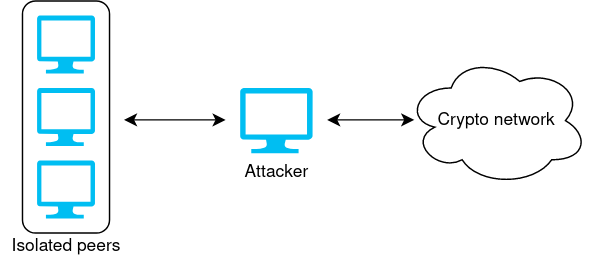
\includegraphics[width=.55\textwidth]{pict/network-partition.png}
	\centering
	\caption{Network partition}
	\label{fig:net-part}
\end{figure}


\section{Sybil attack}\label{sec:sybil}
In a Sybil attack a malicious user controls multiple identities on the network that can be either real machines or dummies, fake replicas of the attacker~\cite{douceur2002sybil}.

Such vector of attacks is applicable to any peer-to-peer system where users can create an arbitrary number of identities on the network for there is no node identification mechanism~\cite{kedziora-sybil-ledgers}. Thus, Bitcoin can suffer from such attacks.

Although the creation of fake identities cannot be exploited to carry out 51\% attacks, since they do not hold any computing power, they can still be used to spread forged information or to withhold blocks.

In the latter scenario, Sybil nodes, upon receiving a new block, send \texttt{inv} messages to their neighbours, but then leave unanswered the following \texttt{getdata} messages, thus delaying the propagation of blocks, as shown in \emph{Fig.~\ref{fig:sybil}}.

\begin{figure}[h!]
	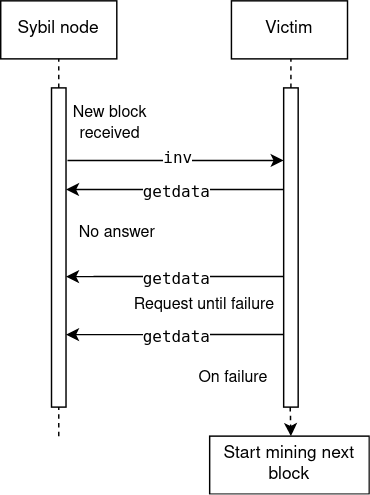
\includegraphics[width=.4\textwidth]{pict/sybil.png}
	\centering
	\caption{Sybil nodes behaviour during the attack}
	\label{fig:sybil}
\end{figure}

If the propagation is delayed long enough, the victim node could start mining the next block - in such scenarios a block race can be engineered. Block races occur whenever the blockchain is forked and different subsets of peers work on different branches of the chain.

Since only the longest chain stored among all peers is considered valid, all the other branches are dropped. The malicious user can exploit such forks to waste other peers' computing power or to perform double-spending~\cite{zhang-ds-sybil}. 

In the latter scenario, once the malicious user has successfully created a stale view of the blockchain in the victim, i.e. a fork, he releases two different transactions, Tx 1 and Tx 2, at the same time. Tx 1 is sent only to the victim node and Tx 2 is kept for its private chain, as shown in Fig.~\ref{fig:race1}.

In the meanwhile Sybil nodes hamper the growth both of the public and victim's blockchain by withholding blocks. As a result the attacker can mine the next block first and then release the private blockchain therefore invalidating the victim's blockchain, as shown in Fig.~\ref{fig:race2}.

\begin{figure}[h!]
	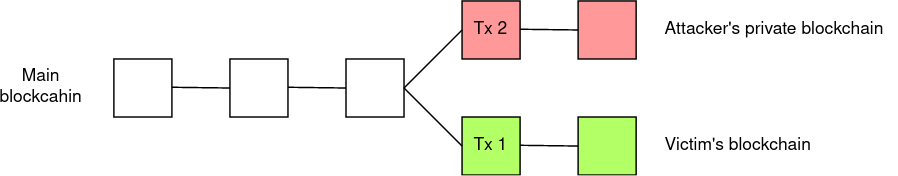
\includegraphics[width=.9\textwidth]{pict/blockrace1.png}
	\centering
	\caption{Block race for double-spending}
	\label{fig:race1}
\end{figure}

\begin{figure}[h!]
	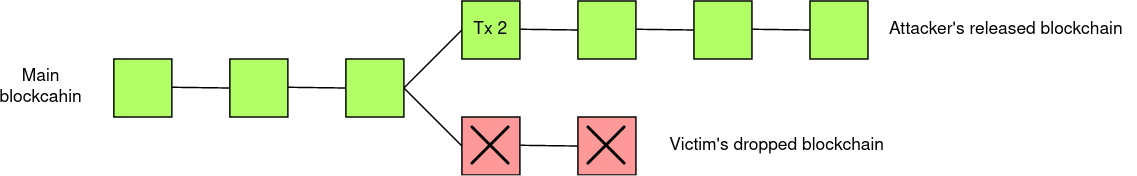
\includegraphics[width=.9\textwidth]{pict/blockrace2.png}
	\centering
	\caption{The attacker releases the longest chain}
	\label{fig:race2}
\end{figure}

Since Bitcoin requires no authentication or authorization to join the network, there will always be the possibility for adversaries to create Sybils. Nevertheless, countermeasures have been studied for different attacks based on Sybil attacks. For instance, setting a transaction block-confirmation timeout has been suggested by Zhang et al.~\cite{zhang-sybil-mitigations}.

Be that as it may, the implications of Sybil attacks are still a topic open to study. The interested reader can find more in the work of Iqbal et al.~\cite{iqbal-sybil}.

\section{Eclipse attack}\label{sec:eclipse}
The aim Eclipse attacks is to partition the network so that the attacker may be able to control all the data flowing between the two partitions.

In order to do that the malicious node, or a set malicious nodes, floods the victim with a multitude of incoming connections and feed it bogus network information, i.e. peer addresses controlled by the adversary, with \texttt{addr} exchanges, that will fill up their peer cache.

Upon restarting, with high probability the victim will form all of its eight outgoing connections with malicious IP addresses, thus finding itself isolated from the network.

Successful Eclipse attacks enable mining and spending attacks. Namely, eclipsing a subset of peers eliminates their mining power, hence making 51\% attacks easier. Selfish mining attacks can be carried out as well.

The attacker that successfully splits the network can also engineer block races to deliberately waste resources of other miners or attempt at double-spending attacks, as in Fig.~\ref{fig:race1} and Fig.~\ref{fig:race2}, described in Section~\ref{sec:sybil}.

Depending on the victim's policies, the malicious user can launch a \textit{0-confirmation double-spending attack}, that is for the case in which the merchant decides to release goods before the transaction is confirmed. As in the case of Sybil based double-spend, the attacker releases two transactions and keeps the victim's view of the blockchain stale, so that it would be dropped later (Fig.~\ref{fig:0confirm}).

Compared to the Sybil-based double-spending, Eclipse-based double-spending attacks of this kind have a greater chance of success, since they control all the victim's traffic and do not have to rely on delaying a block from spreading. Although the attacker needs to go through the partition set up first, whereas creating sybils is much easier.

\begin{figure}[h!]
	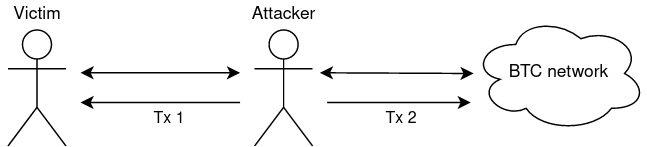
\includegraphics[width=.7\textwidth]{pict/0confirm-doublespend.png}
	\centering
	\caption{0-confirmation double-spend}
	\label{fig:0confirm}
\end{figure}

Were the victim to adopt a N-blocks confirmation policy for transactions, the attacker can still launch a \textit{N-confirmations double-spend} if it successfully eclipsed a subset of connected peers.

If that is the case, then the victims can be kept on an arbitrarily stale view of the blockchain and then be given one of the two transactions the attacker creates, while giving the other to the rest of the cryptocurrency network. After the eclipsed peers mine $N - 1$ blocks, the transaction is confirmed and the goods are exchanged. Thereafter, the obsolete branch of the blockchain known by the victims will be dropped once the attacker releases the up-to-date (and longer) version disseminated in the network (Fig.~\ref{fig:nconfirm} describes the process).

\begin{figure}[h!]
	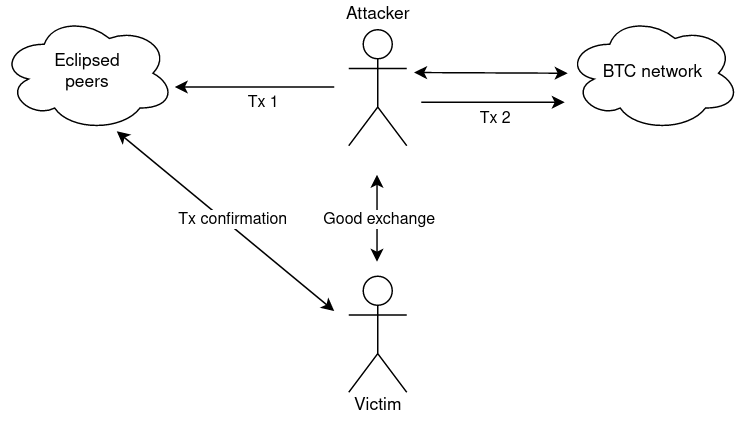
\includegraphics[width=.75\textwidth]{pict/nconfirm-doublespend.png}
	\centering
	\caption{N-confirmation double-spend}
	\label{fig:nconfirm}
\end{figure}

In 2015, Heilman et al. widely describe eclipse attacks and suggest many countermeasures to harden the network, a few of which were implemented in Bitcoin Core~\cite{eclipseatk}. As part of the adoption of these countermeasures, the number of buckets in \texttt{new} and \texttt{tried} has been increased, the addresses have become deterministically hashed to a single slot inside a bucket and the heavy bias towards addresses with fresher timestamps when choosing new connections has been removed.


\section{Fake bootstrapping attack}\label{sec:fakeboot}
Every peer-to-peer system needs some mean to let nodes join the network: in Bitcoin bootstrapping nodes need to rely on the information provided by some other peer in the network.

In a fake bootstrapping attack the peers contacted while a node is still initiating its connections, and hence its knowledge of the network, flood the bootstrapping peer with malicious addresses.

The results in Chapter~\ref{sec:res} show how feeding bogus information to a joining node can seriously influence its view of the network and lead to network partitions and peer eclipsing. This condition would also increase the efficacy of other network-level attacks, such as a DDoS, and the success rate of spending and mining attacks~\cite{eclipseatk}.\\

Prevention is done by ensuring a node can contact a trustworthy peer when joining the network. Peer caches and centralized bootstrap services serve this purpose, allowing joining nodes to make use of old neighbours while having central bootstrap servers as a fallback.

Other solutions have been implemented and tested over time, though their drawbacks usually exceed the benefits. As an example, randomly probing the address space, scouting for peers, decentralizes the bootstrap process and increases the variance of the network knowledge, but may not work if peers are behind NATs or firewalls and increases the latency for joining the network~\cite{decentrbootstrapp2p}~\cite{localityaware}.

In 2012,  Touceda et al. discuss fake bootstrapping along with other security threats in their survey~\cite{toucedafakeboot}.

Bitcoin employs many countermeasures, and overcomes other bootstrap issues, with its peer cache implementation mixed with external mechanisms: each node contacts its stored addresses for successive connections and aims to establish multiple outgoing connections, thus it does not rely on a single bootstrap node.

On top of that, DNS seeds provide a reliable external bootstrap service and the user is given the ability to manually insert addresses to connect to~\cite{mahmoud_netsec_boot}.